% !TEX root = ../main.tex

\section{Introduction}
% Why is this important.
% PAPER BEING SOLD HERE
%______________________________________________________________%

\section{Preliminaries}

\subsection{What is Front running?} %Definition of frontrunning
\label{sec:What is frontrunning?}

\emph{Front running} is analogous to any course of action during which a person benefits from prior access to inside or confidential market information to upcoming transactions and trades. This problem can occur in both financial and non-financial systems, however, it is more noticeable within the trading and exchange systems as it was originated back in stock markets. In the old times, all the trades were executed on papers, so in case of receiving a large order from a client, the broker might say this loud and other people around the table could be informed. Therefore, a malicious trader would now run in front of that order and put his own transaction in between (before the trade was executed) and profit from the price increase of the stock. In other words, a group of market participants obtain non-public market information which allows them to front-run other users trades by putting their orders a head of those trades and benefit from advance knowledge of pending client orders. The two significant factors which cause the front-running practice to happen within the financial markets are (i) imperfect competition and (ii) liquidity uncertainty. \textbf{should I explain more?!} Any sort of front-running activity within the financial markets is considered as an unethical and illegal practice as it is unfairly beneficial for a few market participants who have the privilege of acting on this information and taking advantages at the expense of the investor. 



\subsection{Front Running on the Blockchains}
\label{sec:Front Running on the Blockchains}

Blockchain technology has received an exceptional amount of attention since it was first introduced as the underlying technology of the cryptocurrency Bitcoin in Satoshi Nakamoto's (pseudonymous) 2008 white paper \cite{nakamoto2008bitcoin}. Many decentralized applications that are nowadays built on top of this technology represent the significance of the blockchain as it completely eliminates the single points of failures within any systems. However, blockchains have some inherent characteristic that leave them vulnerable to \emph{front running} behaviour. Although this data structure is known to be publicly visible to every network participants, information is layered  and some of them are accessed only by insiders. Any network participants that runs a full node on the blockchain is able to obtain those information and as mentioned in Section~\ref{sec:What is frontrunning?}, this leaves the application vulnerable to front running. Decentralized exchanges are a group of blockchain financial applications where front running can be executed. Bancor \cite{hertzog2017bancor} is an example of such systems in which front runners benefit from potential price increase of the market stocks (details are provided in Section ...). Decentralized namespaces, as blockchain non-financial applications, are another example. Ghazal \cite{moosavighazal} is such system in which upon seeing a transaction from Alice to register \texttt{alice.com}, front runner can go ahead of her and register this domain name. He can later sell \texttt{alice.com} to Alice for a higher price and benefit from the price increase.
Another application that is vulnerable to front running is Initial Coin Offering, ICO, smart contracts. ICO is a method to distribute tokens based on the deposits of the native coin, Ether in the case of Ethereum. After a few hacking incidents on high valued smart contracts~\cite{siegel2016daohack}, ICOs started to implement restrictions and capped how much funds can be gathered. This scarcity of the initial coins made for a competition to incentivize big investors to get in and buy the tokens at a discounted price and sell them to late comers on the open markets~\cite{zetzsche2018ico, li2018initial}. ICOs started to experiment with different fair capping methods, such as reverse dutch auction, dynamic ceilings, \eg ~\cite{kaal2017initial}.  This competition made ICOs a good opportunity for frontrunning attacks. 


%___________________________________________________________%

\section{Related Work}
As the traditional frontrunning was originated to trading financial instruments most of the literature are focused on financial aspects of the markets. %TODO: expand this with something


\subsection{Historical Context / Classic Frontrunning}
Frontrunning was first appeared on the Chicago Board Options Exchange ( \textit{CBoE}) ~\cite{markham1988front}, and was identified by \textit{Securities Exchange Commission} in 1977 as the following:
\begin{quote}
The practice of effecting an options transaction based upon non-public information regarding an impending block transaction\footnote{Block in the stock market is large number of shares, 10\,000 or more, to sell which will heavily changes the price} in the underlying stock, in order to obtain a profit when the options market adjusts to the price at which the block trades. ~\cite{sec1978optionsmarket}
\end{quote} 

%In actuality, front-running is more complex than this definition suggests. It encompasses at least three forms of conduct, each of which raises different regulatory and policy issues.9 They are: (1) trading by third parties who are tipped on an impending block trade ("tippee" trading); (2) transactions in which the owner or purchaser of the block trade itself engages in the offset- ting futures or options transaction as a means of "hedging" against price fluctuations caused by the block transaction ("self-front-running"); 1 ° and (3) transactions where a broker with knowledge of an impending customer block order trades ahead of that order for the broker's own profit ("trading ahead").
% from JerryWMarkhamFrontRunning.pdf

% More to read and add from : SECURITIES AND EXCHANGE COMMISSION Release No. 34-67079. pdf included in Related_Documents
% https://www.sec.gov/about/annual_report/1988.pdf

On the years after there were ongoing discussions between self-regulatory exchanges (\eg \textit{CBoE}) and  \textit{SEC} to regulate, detect and define laws and regulations to deal with frontrunning~\cite{markham1988front}, with \textit{SEC} stating: 
\begin{quote}
It seems evident that such behaviour on the part of persons with knowledge of imminent transactions which will likely affect the price of the derivative security constitutes an unfair use of such knowledge. \footnote{Securities Exchange Act Release No. 14156, November 19, 1977, (Letter from George A. Fitzsimmons, Secretary, Securities and Exchange Commission to Joseph W. Sullivan, President  CBoE).}
\end{quote} 

As defining what exactly is considered illegal front-running required more knowledge of how these new markets behave, \textit{CBoE} and other exchanges (and brokers) issued educational circulars for their members asserting that frontrunning violates existing rules, with some examples of what is considered frontrunning. However difference of opinion regarding the unfairness o front running activities, insufficient exchange rules and lack of a precise definition in this area resulted in no action by self-regulator organizations~cite{sec1978optionsmarket}. 

Further reading on the early details on the history and challenges of detecting and regulating frontrunning can be found in~\cite{markham1988front} . % TODO: add a more recent publication here as well! 

Initially the frontrunning policies only applied to certain option markets, later on in 2002, the rule was refined to include the same prohibitions to security futures~\cite{finra_2002}, which then in 2012 with the new amendment, FINRA Rule 5270, the frontrunning rule was extended to cover trading in an option, derivative, or other financial instruments overlying a security with some exceptions~\cite{sec2012frontrunning, finra_2012}. 


\subsection{Recent Literature on Blockchain frontrunning}

~\cite{malinova2017market}
~\cite{aune2017footprints}
~\cite{breidenbach2018enter}


% NOTE: use double-spend paper (first)
% talk about double-spend one kind of frontrunning (relationship between frontrunning vs double spend) rushing actors. 
% Double-spending fast payments in bitcoin.pdf


%______________________________________________________________%


\section{(On) Blockchain Front-running}

\subsection{Who Can Front-run?}
\label{sec:who can frontrun?}

In general, all the network participants have the ability to front run specific transactions that are sent to the network. However, miners can include any transactions they like into the block they attempt to mine. Thus, they possess special power in terms of front running as opposed to other users of the network. In the following, we discuss and compare the two groups of blockchain potential front runners.

\subsubsection{Miners}
As mentioned above, since the Blockchain miners are the only parties who can decide on the order of transactions within a block they mine, they can easily intercept and reorder the pending transactions sitting in the mempool and profit from a guaranteed price-rise. For example in an Ethereum based application, a miner learns about the pending \textit{buy} transaction of 1000 units of a token, i.e. TKN, presumably if this transaction goes through, it causes the price the purchased token to increase. So the dishonest miner can step in front of this transaction and  place his own buy order ahead of it. He would simply create his \textit{buy} of 1000 TKN and include it within a block and now he mines the previous \textit{buy} transaction of 1000 TKN. Doing so, he would receive a better rate than other network users, and can sell the assets he has received and gain a price advantage at the expense of others. Similarly, a dishonest miner can sell his tokens in front, if he sees a pending \textit{sell} transaction. In an open source blockchain application, there is no rules on how transactions must be ordered and miners are free to send transactions in the order they prefer. However, miners can only front run other transactions (by reordering them) within the block they happen to mine. They could do this also by not broadcasting their own transactions to the network, this makes the miners to be less noticeable to the network when front running.
Another example here is in the case of decentral exchanges and order cancellation. Every exchange should have the functionality to cancel the orders, especially for a volatile market. In this case, when user decides that her order is not profitable anymore, she would send a cancelation transaction. Here the miner sees the cancelation transaction and puts his own order before the cancellation transaction to fill the order, potentially profiting from the order. They can also include the canceled transaction in their block to collect the full gas limit used by that transaction~\cite{CostofDecentralization:online}.


\subsubsection{Blockchain users/nodes}
Any regular (non-miner or miner) user can also front-run other transactions in the network. For regular users to front run others on the blockchain, they need to be fully/well connected to other nodes on the network. Doing so, they are able to listen to the network and monitor all transactions that are broadcast. On the Ethereum blockchain users have to pay for the computations in small amount of Ether called \textit{gas}~\cite{AccountT67:online}. The price that users pay for transactions (a.k.a. transaction fees) can increase or decrease how quickly miners will execute them and include them within the block they mine. This is because the Ethereum miners consume resources to process the transactions and so receive the transaction fees after creating the blocks. Once seeing two identical transactions with different transaction fees, 
%Given the limited space in the blocks, a rational miner will prioritize transactions that pay higher gas price per unit of gas, this maximizes their profit in the block they mine.
miners act to maximize their profit and are free to mine the transaction which offers the highest fee. Therefore, any regular users who run a full-node Ethereum client can modify the order of pending transactions by paying with a higher gas price\ie by monitoring the network, upon seeing a  pending \textit{buy} transaction which will further increase the price of the asset, a font-runner user can pay a higher gas price and hope to have his transaction a head of the other one mined. By doing so, he achieves a better rate from the other network users. Note that in this case, blockchain front runners are more visible to the network as they broadcast their transactions to all the network participants. 


%\subsubsection{Blockchain users/nodes}:
%\begin{itemize}
%\item{\textbf{Higher GasPrice}: Monitor transactions, rebroadcast with higher GasPrice}
%\item{\textbf{Fully/well connected nodes}: Similar to HFT situation of faster connections to other nodes, for a higher chance of transaction inclusion, also Sybil attacks?} 
%\item{\textbf{Noticable by the network}: More visible to the network as both transactions are broadcast to all the nodes}
%\end{itemize}
%
%
%\subsubsection{Miners}
%
%
%\begin{itemize}
%\item{\textbf{Their own mined blocks}: The can only frontrun transactions within the block they mine. This could be done by reordering the transactions within the blocks.}
%%^ If a miner or user sees an unconfirmed transaction in the mempool they could squeeze their own transaction to come in front and profit from that. Essentially, profitting from reordering the transactions.
%
%\item{\textbf{Less Noticable by the network}: Miners can include transactions within the blocks they happen to mine without broadcasting the transactions, hence less chance of being detected by the network participants.} 
%%Should the following be included? 
%%\item{\textbf{Incentivized mitigation methods}: applications could pay the fees to the miners to incentives them to behave } 
%\end{itemize}


\subsection{Historical evidence in the Blockchain}
As blockchain records are immutably recorded, there is enough historical data to analyze for possible front running detection. For examples here we research some of the events of such attacks happening in the Ethereum blockchain applications.

% maybe inlcude 0xbitcoin ERC721 mineable tokens frontrunning!
% mint: https://etherscan.io/tx/0x9883bc3ad018fd2b649982f88fbad7dc5abcb8f11c4f1d87ef814ba30c2b3428

\subsubsection{Status ICO} \hfill\\ 
\noindent As discussed in ~\ref{sec:Front Running on the Blockchains}, capped ICOs are a good application for frontrunning attacks.  In June 2017, Status.im~\cite{statuswhitepaper} started their ICO and within 3 hours they reached their cap, resulted in close to 300,000 Ether of funding. They used a \textit{fair} token distribution method called \textit{Dynamic ceiling}, which was in place to prevent large investments to take place early and limited the amount of Ether deposited, this was an attempt to increase the time window for smaller investors. They implemented multiple caps --ceiling-- which each would have a maximum amount that can be deposited. In this case every deposit would be checked by the smart contract and the exceeding amount would be refunded to the sender while the accepted amount would be sent to the Status.im wallet ~\cite{statusicoanalysis}. 
On the time of the ICO there were reports of Ethereum network being unusable and transactions were not confirming. Further study showed that some mining pools might have been manipulating the network for their own profit.

\begin{figure}[h]
\centering
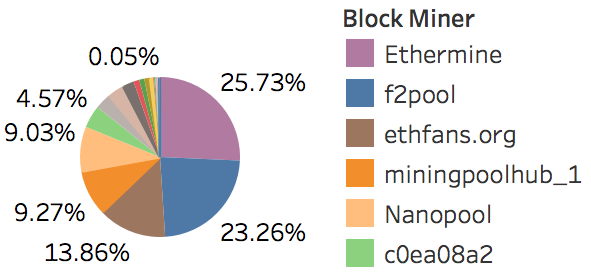
\includegraphics[width=0.5\linewidth]{figures/Mining_pool_ratio.png}
\caption{The percentage of Ethereum blocks mined between block 3903900 and 3908029, this is the time frame in which Status.im ICO was running. This percentage roughly shows the hashing power ratio each miner had at that time. \label{fig:mining_pool_ratio}} % IS THIS STATEMENT CORRECT?
\end{figure}

F2Pool, an Ethereum mining pool that had around 23\% of the mining hash rate at the time (Figure ~\ref{fig:mining_pool_ratio}), sent 100 Ether to 30 new Ethereum addresses before Status.im ICO started. On the time the ICO started F2Pool constructed 31 transactions from the addresses they controlled to the ICO token sale smart contract --without broadcasting these transactions to the network-- and focused their mining power to mine their own transactions.
As shown in figure  ~\ref{fig:Transactions_miners_while_status_ico_cut}, most of the top miners in the mentioned time frame, have mined almost the same number of failed and successful transactions which were directed toward Status.im token sale, however F2Pool's transactions indicate their successful transactions were equivalent to 10\% of the failed transactions, hence maximizing the mining rewards, on gas, while censoring other transactions to the token sale smart contract.


\begin{figure}[h]
\centering
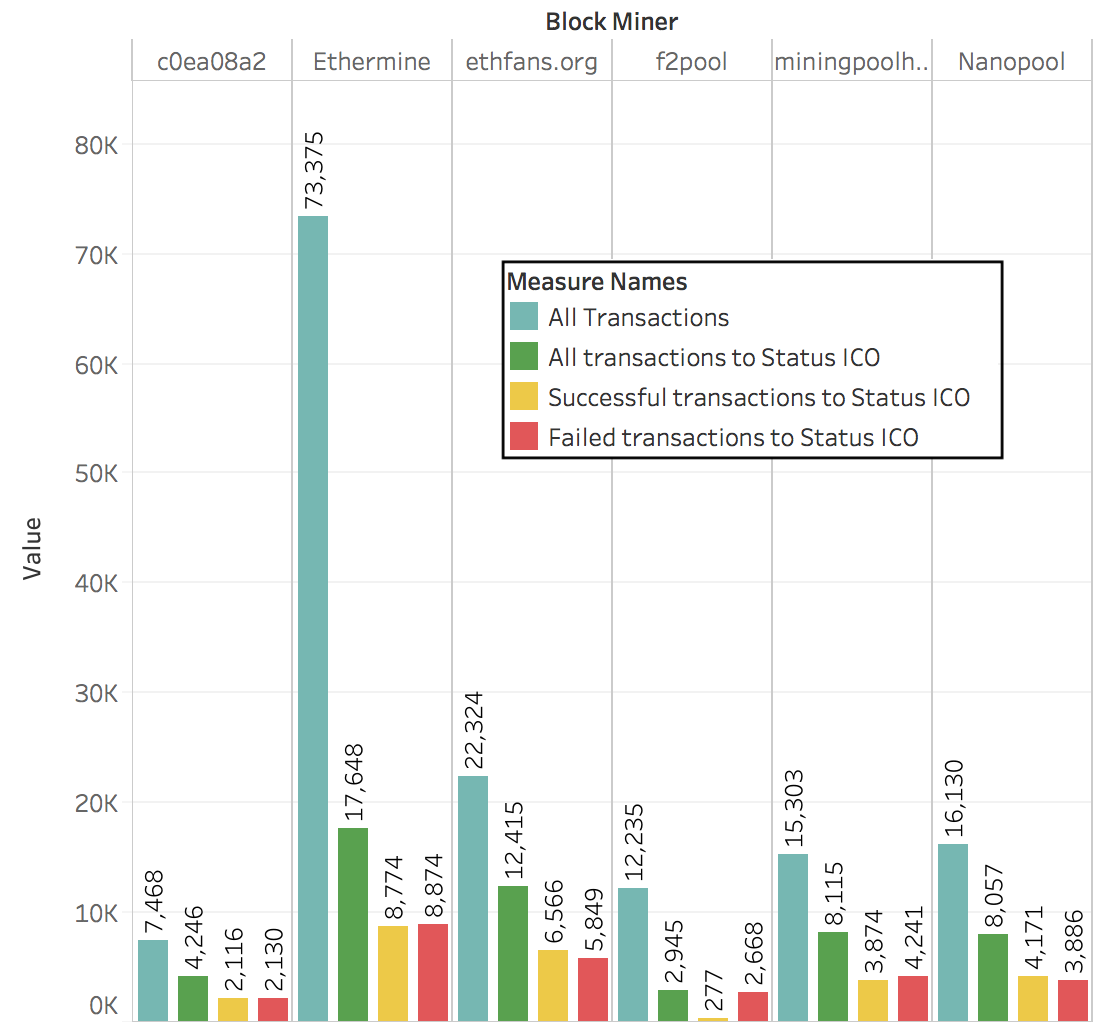
\includegraphics[width=0.7\linewidth]{figures/Transactions_miners_while_status_ico_cut.png}
\caption{This chart shows the miner behaviour on the time window that Status.im ICO was running. \label{fig:Transactions_miners_while_status_ico_cut}} 
\end{figure}


Involvement of F2Pool in this action becomes obvious when the transactions from these 30 addresses are traced. As shown in figure ~\ref{fig:f2poolfrontrun}, the funds deposited by F2Pool in these addresses where sent to Status.im ICO and mined by F2Pool. Once the dynamic ceiling algorithm refunded a portion of the sent funds back to these addresses, these funds were again sent back to F2Pool main address. 


\begin{figure}[h]
\centering
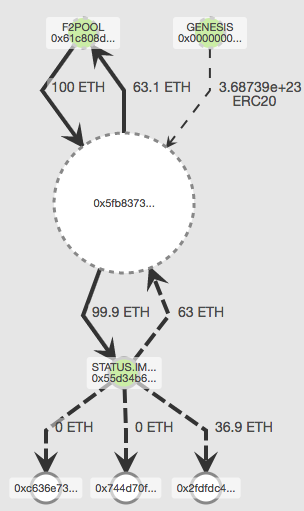
\includegraphics[width=0.7\linewidth]{figures/F2Pool_transactions_to_StatusICO_and_Refunds.png}
\caption{F2Pool prior to Status.im ICO deposited 100 Ether in multiple new Ethereum addresses. On the time of the ICO they sent these deposits to Status ICO smart contract and prioritized mining of these transactions in their mining pool, this was to overcome the dynamic ceiling algorithm of the token sale smart contract. Later on they sent the refunded Ether back to their own address.\label{fig:f2poolfrontrun}}
\end{figure}


Although this incident does not involve transaction reordering in the blocks, it shows how miners can modify their code to behave in centain way that could result in their monetary profit. 
%TODO: these might need more details and proofs. ask Jeremy about how to go on about this! 


%Also the ICO smart contract only accepted transactions with gas price lower than 50gwei, unless they were whitelisted before. this was for preventing high gas payers to get in front of the line. although as this was not clearly communicated to users (UX issues?), there were tons of transactions that failed due to high gas price but also clogged the ethereum network as the miners chose transactions with higher gas price to be included in their blocks.



%What is Bancor and how it can be frontrun:%
\subsubsection{Bancor} \hfill\\
\noindent Bancor is an Ethereum-based application that allows users to exchange their tokens without any counter-party risk. This protocol aims to solve the cryptocurrency liquidity issue by introducing \textit{Smart Tokens}~\cite{hertzog2017bancor}-- ERC20 compatible tokens with a built-in liquidity mechanism that are always available to users. Smart Tokens can be bought and sold through the users smart contract at an automatically calculated price which displays supply and demand. Doing so, Bancor protocol provides continuous liquidity for digital assets without relying on an order book as there is no requirement to match sellers and buyers.

\par\noindent\textbf{Front-running Bancor} Recently, researchers have shown that Bancor is vulnerable to front running attacks. Implemented on the Ethereum blockchain, when Bancor transactions are broadcast to the network, they sit in a pending transaction pool known as \textit{mempool} waiting for the miners to mine them. Since Bancor handles all the trades and exchanges on the Ethereum blockchain (unlike other existing decentralized exchanges), these transactions are all visible to the public for 16s (the average Ethereum blocktime) before being included within a block. This leaves this blockchain-based decentralized exchange vulnerable to the blockchain race condition attack as attackers are given enough time to front-run other transactions and gain favourable profits~\cite{BancorIs7:online}. As mentioned in Section~\ref{sec:who can frontrun?} and same as every other Ethereum based application, Bancor transactions can be front run by miners and other regular (non-miner) users. There is an implementation of a Bancor front running attack in the Python programming language which represent how a non-miner user can front run other network participants \cite{NewTab13:online}.




%\begin{itemize}
%\item {\textbf{Miner Frontrunning.}} As mentioned, Bancor protocol uses an algorithm that automatically calculates the price of digital assets to provide better market liquidity. In the Bancor model, essentially buy orders increase the price of the tokens while sell order decrease it. Since the Blockchain miners are the only parties who can decide on the order of transactions within a block, they can easily intercept and reorder the pending transactions sitting in the mempool and profit from a guaranteed price-rise. For example, a miner learns about the pending \textit{buy} transaction of 1000 Ether, based on the Bancor design, if this transaction goes through, it causes the price of Ether to increase. So the dishonest miner can step in front of this transaction and  place his own buy order ahead of it. So he would simply create his \textit{buy} of 1000 Ether and include it within a block and now he mines the previous \textit{buy} transaction of 1000 Ether. Doing so, he would receive a better rate than other Bancor user, can sell the tokens he has received and gain a price advantage at the expense of others. Similarly, a dishonest miner can sell his tokens in front, if he sees a pending \textit{sell} transaction.
%
%
%\item {\textbf{Non-miner Frontrunning.}} Researchers have also shown that a regular non-miner user can also front-run Bancor. In order for the Bancor transactions to be executed on the Ethereum Virtual Machine (EVM),  users have to pay for the computations in small amount of Ether called \textit{gas}~\cite{AccountT67:online}. The price that users pay for transactions (a.k.a. transaction fees) can increase or decrease how quickly they are executed and included within the blocks by the miners.  This is because the Ethereum miners consume resources to process the transactions and so receive the transaction fees after creating the blocks. Once seeing two identical transactions with different transaction fees, profit maximizers miners are free to mine select the transaction which offers the highest fee. Therefore, any regular non-miner users who run a full-node Ethereum client can modify the order of pending transactions by paying a more amount of gas \ie by monitoring the network, upon seeing a  pending \textit{buy} transaction which will further increase the price of the asset, a font-runner user can pay a higher gas price and send his transaction a head of that. By doing so, he achieves a better rate from any other Bancor users.
%
%\end{itemize}


%NOTE: @mahsa: is this considered a Historical evidence? should we talk about this somewhere else and maybe do a PoC on Ghazal for this section?
\subsubsection{Domain Name Front-running} \hfill\\    %Following section talks about frontrunning in namespaces but limited to Ghazal. Will talk about NameCoin in the section of mitigations (commit & reveal method)
\noindent As mentioned in Section~\ref{sec:Front Running on the Blockchains}, although front-running attacks have been more showcased in the context of decentralized exchanges and trading systems, they are are not yet limited to the financial markets. Front-running can occur within other (non-financial) blockchain applications such as naming systems. Blockchain-based domain registrar have been introduced to eliminate the role of central parties \ie domain name system (DNS) which introduce single point of failures in the entire web. One such system is Ghazal, an Ethereum-based naming and PKI system~\cite{moosavighazal}. Ghazal users rely on the Ethereum blockchain to register their \texttt{.ghazal} domain names and bind certificates to those names. In Ghazal model, a user would register domain name by executing the \textit{registerdomain} function from the Ghazal smart contract with the domain name in plain text as the function argument. As mentioned before, These transactions will sit in the mempool so that it would be mined by Ethereum miners and included in the block. During this period in which the transaction is not yet confirmed, front-running attack can occur by (i) dishonest miners and/or (ii) regular non-miner user. In the first case, a miner would intercept the \textit{registerdomain} transaction and register that name ahead of the user. A regular non-miner node in the Ethereum network can front-run other user's \textit{registerdomain} at a good profit by paying higher transaction fees. This practice allows the adversarial party  to register an unregistered domain immediately after someone searched for it, and sell the domain name to the users for a higher price. Note that, domain name front-running also occurs in the vanilla system. In this case, front-runners would monitor and identify domain names of interest, and sell it back to the other users with a higher price~\cite{sac022en33:online}.
% PoC of frontrunning ghazal
%TODO: also talk about ENS 



%______________________________________________________________%




\section{How to stop frontrunning?}
In the traditional markets, frontrunning is considered unethical and also illegal. In the blockchain space, the designers of the decentral applications cannot rely on the justice system for unethical behaviour, and they must assume that each participant in the network acts rationally in their own self interest, the application will be operating in an adversarial environment~\cite{0xfrontrunning:online}.
A few decentral exchange projects such as \textit{EtherDelta} and \textit{0xProject}~\cite{warren20170x}, have proposed solutions for frontrunning, which is off-chain orderbooks. The methods discussed within these projects prevent blockchain network participants from front running the orders as the orders are private and not known to the network and will not be broadcasted. However they are introducing third parties, \eg relayers in 0xproject, to be managing the orders with the promise not to reorder or frontrun other orders. 

\emph{Traditional Frontrunning Prevention Methods}. regulations/enforcement/broker education/sealed order
%@shayan: ^


\emph{Blockchain Frontrunning mitigation/prevention}. The traditional methods of preventing frontrunning are based on regulation and restrictions applied to the brokers and actors within the markets, such methods do not apply to blockchains, no enforcement methods, ... 

There are two main approaches to prevent front running, one to design a blockchain that is frontrun-resistent , and the other to design the application logics in a way that front running is not possible. 


\subsection{Frontrun-resistent Blockchain}
What does this mean to have a frontrun-resistent blockchain?  There are technical difficulties to achieve such solutions as there are unknown factors within such network designs (corner/edge cases).

\begin{itemize}
\item{\textbf{Privacy Preserving Blockchians}: Shielded transactions in ZCash do not reveal the sender, receiver, the amount and the data included in the transactions, hence they cannot be seen by network participants to be frontrunned. Although this limites the functionality of the blockchain/smartcontracts/dapps }
\item{textbf{Loopring/Dual Athoring}: Talk about this possible solution}

\end{itemize}


\subsection{Application Design to Prevent Front-running}

Another way of preventing the front-running activities is to design the applications, whether they are decentralized (Dapps) or centralized, in such a way that no information would be available to the malicious parties which enables them to front-run the other users.
Followings discuss the two techniques which can be used by the Apps/DApps developers while designing the systems to prevent front-running activities.

\begin{itemize}
\item{\textbf{Commitment scheme}: Also known as \textit{Commit and Reveal}, is a cryptographic primitive that enables one to commit to a value (\eg statement, document, \etc}) while keeping it a secret and on a later time reveal the committed value~\cite{brassard1988minimum}. Commitment scheme is a good method to prevent information leakage from the sensitive transactions. This could be done by simply broadcasting the hash value of the committed data and later on revealing the values that would be hashed to the committed hash. 
In the case of decentral exchanges, user can send a commit transaction which will be cryptic to network participants but will act as a placeholder in the queue for the user, after the transaction is mined, user sends reveal transaction revealing the order details which will be executed in a fair order. Another use of such commitment scheme, is in decentralized naming systems, such as Ghazal or ENS. In this case, a user would send a commit transaction similar to a sealed bid, once the transaction is confirmed and the grace period is over, user would send a reveal transaction revealing the bid and also the details of the requested domain. Using this scheme, one is able to hide information from the adversarial parties in the system and prevent them from front-running.


%TODO: a figure for commit and reveal? 

%although it does not hide the participatory factor (it shows the actor participated in the application but hides the details, obvious participation(commit))}
% discussion about Anonymity-set ?


\item{\textbf{Submarine sends}: describe. General solution similar to commit and reveal. This is to solve the participatory factor of the commit and reveal solution.}

\item{\textbf{Application logic specific solution}: Depending on the use case of  the Dapp or the application, it could be designed in a way to deincentives some actors to frontrun the transactions or prevent them from doing so. As an example on desiging a decentral orderbook, it could be said that a miner could front run orders for financial gain on price improvement, however if the fees of the orders are sent to the miner of the block, it deincentiveses the miner to front run the orders as they already gain enough financial benefit from including the correct order of transactions. 
Another example for decentral orderbook design could be using call market design instead of  time-sensitive orderbooks. In such design the arrival time of the order does not matter as they are executed in batches. }

%Proof of burn methods ? 

\end{itemize}



%______________________________________________________________%




\section{Concluding Remarks}


% Could talk about a tool / a framework to detect frontrunning


%\subsubsection*{Acknowledgements.}
